\subsection{Version naïve}
Pour implanter la version mémoire partagée, nous construisons l'architecture dans
\iCode{CentralizedLinda} ci-dessous, on fait une première version sans se préoccuper
d'\iCode{eventRegister}. Les interfaces et classes \iCode{Linda}, \iCode{Tuple},
\iCode{Callback}, \iCode{AsynchronousCallback} sont figées et ne doivent en aucun cas être modifiées.


\begin{figure}[H]
    \centering
    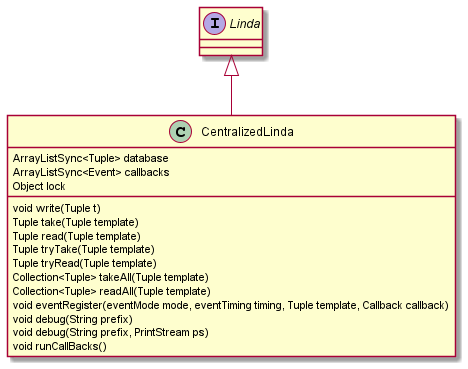
\includegraphics[scale=0.7]{src/part-02/src/fig-2.png}
    \caption{CentralizedLinda} \label{fig:centralized-linda}
\end{figure}

Pour l'\iCode{eventRegister}, on fait l'algorithme ci-dessous :

\begin{dinglist}{111}
    \item On met en réserve le \textit{callback}
    \item Si \iCode{timing} vaut \iCode{immediate}, on supprime le \textit{callback}
\end{dinglist}

\codeFromFile{java}{src/part-02/src/eventRegister.java}{CentralizedLinda.eventRegister}{event-register}

\subsection{Version multithreadée}
